\documentclass[11pt,a4paper]{article}
\usepackage{myStyle}

% Set absolute file path for project
% Change to approriate path when starting project.
\newcommand{\projectpath}{/home/joanna/Dropbox/Sketchbook/python/project_template}

\usepackage{fancyhdr}
\pagestyle{fancy}
\renewcommand{\headrulewidth}{0pt}
\fancyhf{}
%\chead{
\includegraphics[width=1cm]{./img/logo.png}}
%\setlength\headheight{28pt} 
\lfoot{Analysis plan version 1, day month year}
\rfoot{\thepage}

% Graphicspath used to avoid trouble with paths. 
\graphicspath{{\projectpath/src/notes/img/}}

\begin{document}

\pagenumbering{arabic}
\setcounter{page}{1}

\section*{Title}
The best study in the world

\section*{Investigators}
Joanna Diong\textsuperscript{1} \\
Agatha Christie\textsuperscript{2} 

\textsuperscript{1}University of Sydney \\
\textsuperscript{2}University of Exeter

% Comment out as required
\section*{Methods}

\subsection*{Aim}

\subsection*{Design}

\subsection*{Setting}

\subsection*{Participants}
Refer to Protocol for details. Briefly, ... 

\subsection*{Procedures}
Refer to Protocol for details. Briefly, ... \citep{Pascoe2014}

\subsection*{Data management and data integrity}

\subsection*{Sample size}

\subsection*{Statistical analysis}

\subsection*{General principles}

\subsection*{Adherence to protocol}

\subsection*{Primary outcome(s)} 
The primary outcomes are: 
\begin{enumerate}
	\item outcome 1
	\item outcome 2
\end{enumerate}

\textbf{Primary analysis}

\textbf{Size of effect}

\textbf{Sensitivity analysis}

\textbf{Missing data handling}

\textbf{Subgroup analysis}

\subsection*{Secondary outcome(s)} 

\textbf{Missing data handling}

\subsection*{Figures and tables}

\begin{figure}[!htbp]
\centering
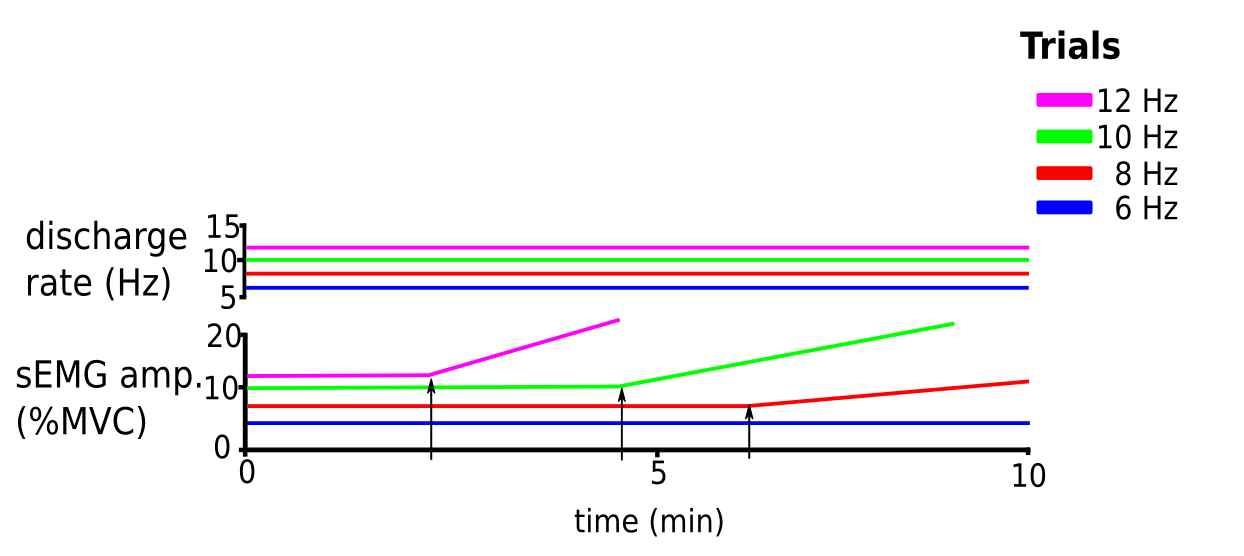
\includegraphics[scale=0.75]{./img/fake_data.png}
\captionsetup{justification=centering}
\caption{Fake data}
\end{figure}

% References:
\newpage
\bibliographystyle{\projectpath/src/ms/refs/jneurophysiol}
\bibliography{\projectpath/src/ms/refs/ref_list}
 
\end{document}
